% A skeleton file for producing Computer Engineering reports
% https://kgcoe-git.rit.edu/jgm6496/KGCOEReport_template

\documentclass[CMPE]{../KGCOEReport}

% The following should be changed to represent your personal information
\newcommand{\classCode}{CMPE 260}  % 4 char code with number
\newcommand{\name}{Andrei Tumbar}
\newcommand{\LabSectionNum}{1}
\newcommand{\LabInstructor}{Moskal}    % The slash is to tell LaTeX that the period is between words
% not sentences so it spaces correctly. It won't appear in the
% final pdf
\newcommand{\TAs}{Jacob Meyerson\\Dennis Lam}
\newcommand{\LectureSectionNum}{1}
\newcommand{\LectureInstructor}{Cliver}
\newcommand{\exerciseNumber}{3}
\newcommand{\exerciseDescription}{Instruction Fetch and Decode Stages}
\newcommand{\dateDone}{March 2nd}
\newcommand{\dateSubmitted}{March 16th}

\usepackage{tikz}
\usepackage{circuitikz}
\usetikzlibrary{calc}
\usetikzlibrary{circuits.logic.IEC,calc}
\usepackage{multirow}
\usepackage{float}
\usepackage{lmodern}
\usepackage{siunitx}
\usepackage{subcaption}
\usepackage{graphicx}
\usepackage[usestackEOL]{stackengine}
\usepackage{scalerel}
\usepackage[T1]{fontenc}
\usepackage{amsmath}

\def\lbar#1{\ThisStyle{%
    \setbox0=\hbox{$\SavedStyle#1$}%
    \stackengine{2.2\LMpt}{$\SavedStyle#1$}{\rule{\wd0}{0.1\LMpt}}{O}{c}{F}{F}{S}%
}}

\DeclareFontFamily{U}{mathx}{\hyphenchar\font45}
\DeclareFontShape{U}{mathx}{m}{n}{ <-> mathx10 }{}
\DeclareSymbolFont{mathx}{U}{mathx}{m}{n}
\DeclareFontSubstitution{U}{mathx}{m}{n}
\DeclareMathAccent{\widebar}{\mathalpha}{mathx}{"73}

\makeatletter
\newcommand{\cwidebar}[2][0]{{\mathpalette\@cwidebar{{#1}{#2}}}}
\newcommand{\@cwidebar}[2]{\@cwideb@r{#1}#2}
\newcommand{\@cwideb@r}[3]{%
    \sbox\z@{$\m@th\mkern-#2mu#3\mkern#2mu$}%
    \widebar{\box\z@}%
}
\newcommand\currentcoordinate{\the\tikz@lastxsaved,\the\tikz@lastysaved}
\makeatother

\newcommand\decbin[9]{%
    \par\smallskip
    \makebox[3cm][r]{$#1$\ }\fbox{#2}\,\fbox{#3}\,\fbox{#4}\,\fbox{#5}\,\fbox{#6}\,\fbox{#7}\,\fbox{#8}\,\fbox{#9}\par}


\def\code#1{\texttt{#1}}

\begin{document}
    \maketitle
    \section*{Abstract}

    In this laboratory exercise, the instruction fetch and decode stages were
    implemented for the MIPS architecture.
    The instruction fetch stage will read from instruction memory at the
    program counter (PC).
    The instruction decode stage is meant to take in an instruction and generate
    control signals as well as data inputs to the ALU and register file.
    This stage will drive the actions of the execute stage later on.
    The exercise was successful as the test-benches created to test the
    output of the fetch and decode stages found no errors in the implementation.

    \section*{Design Methodology}

    \subsection*{Instruction Memory}
    
	Instruction Memory is a large read only block of memory built to hold
	instructions. The memory is byte addressable with an address width of 
	28-bits. This implementation of instruction memory can hold 1024 bytes.
	Any address above the maximum address of 1023 will output zeroes.
	\\

    A read operation at an address will read an entire word (4 bytes).
    The memory was initialized in with bytes in the order that the test-bench
    expected them.
    
    \subsection*{Instruction Fetch}
	
	The instruction fetch stage read from instruction memory at the program
	counter.
	The program counter is an address internal to the instruction fetch stage
	that will increment by 4 on every clock.
	The 4 byte increment is done so that the next instruction can be read.
	
    \subsection*{Instruction Decode}

    The purpose of the instruction decode is to make sense of
    a certain instruction and generate certain control signals.
    Each control signal is sent to a later stage in the architecture
    to select various functionality.
    
    The instruction decode stage holds various components inside of it.
    The register file is instantiated and controlled by the instruction
    decode stage.
    The control unit is implemented to simplify the work done by the decode
    stage and will generate various control signals given an Opcode and function.    
    \\
    
    Table \ref{tab:decode_signals} is shown to describe output signals
    and their purpose is shown.
    
    \begin{table}[H]
        \renewcommand{\arraystretch}{1.2}
        \setlength{\tabcolsep}{12pt}
        \caption{Instruction decode signals and their descriptions}
        \begin{center}
            \begin{tabular}{|c|l|}
                \hline
                Signal & Description\\\hline
                \hline
               	\code{RegWrite} & Set if writing to registers\\\hline
               	\code{MemToReg} & Set if reading from memory\\\hline
               	\code{MemWrite} & Set if writing to memory\\\hline
               	\code{ALUControl} & 4-bit ALU opcode\\\hline
               	\code{ALU} & Set if second ALU operator is coming from immediate\\\hline
               	\code{RegDst} & Determines which register to write to\\\hline
               	\code{RD1} & Read data from address 1 in register file\\\hline
               	\code{RD2} & Read data from address 2 in register file\\\hline
               	\code{RtDest} & Register Rt in instruction (used to propagate destination)\\\hline
               	\code{RdDest} & Register Rd in instruction\\\hline
               	\code{ImmOut} & Sign extended immediate\\\hline
               	
            \end{tabular}
        \end{center}
        \label{tab:decode_signals}
    \end{table}
    
    The control unit implements most of the MIPS instructions including all 
    of the R-type instructions and most of the I-type instructions.
    The missing I-type instructions are the non-word memory instructions
    (\code {lb}, \code{lh}, \code{sb} etc.).
    \\
    One of the signals not fully explained in the table, \code{RegDst}, will select
    between \code{RtDest} and \code{RdDest} to write data to when the instruction
    has finished. The reason \code{RtDest} and \code{RdDest} are required to be
    outputed is because the data is not ready yet (instruction hasn't executed)
    and therefore we need to propagate the potential outputs to a later stage
    and select between the data down the line.
    \\
    Another thing to note here is that the register file is falling-edge triggered.
    This means that the outputs \code{RD1} and \code{RD2} will not update until
    the falling edge where-as the other output signals are updated on the rising edge when the instruction comes in from the fetch stage.
    
    The sign-extended immediate is used when performing I-type instructions.
    All I-type instructions will take in a 16-bit immediate signed number.
    This number needs to be extended to a 32-bit number to input into the ALU.
    To sign-extend, if the most significant bit is \code{1}, the extended bits
    should also be \code{1}.

    \section*{Results \& Analysis}
    \subsection*{Fetch stage}
    To test the implementation of the fetch stage, a test bench was written
    to check the output of the instruction fetch after every clock.
    The instruction memory is initialized with a sequence of 8 words followed
    by zeroes.
    The test-bench will reset the program counter asynchronously to start from
    \code{PC=0}.
    
    The following words were initialized in order in instruction memory
    \begin{table}[H]
        \renewcommand{\arraystretch}{1.2}
        \setlength{\tabcolsep}{12pt}
        \caption{Instruction fetch test cases}
        \begin{center}
            \begin{tabular}{|c|c|}
                \hline
                Address & Value\\\hline
                \hline
               	\code{0x00} & \code{0x11111111}\\\hline
               	\code{0x04} & \code{0x22222222}\\\hline
               	\code{0x08} & \code{0x1f2e3d4c}\\\hline
               	\code{0x0C} & \code{0xaaaaaaaa}\\\hline
               	\code{0x10} & \code{0xbbbbbbbb}\\\hline
               	\code{0x14} & \code{0xcccccccc}\\\hline
               	\code{0x18} & \code{0xdddddddd}\\\hline
               	\code{0x1C} & \code{0xeeeeeeee}\\\hline
               	
            \end{tabular}
        \end{center}
        \label{tab:inst_mem}
    \end{table}

    Behavioural, post-synthing timing, and post-implementation
    timing waveforms were generated.

    \begin{figure}[h!]
        \centering
        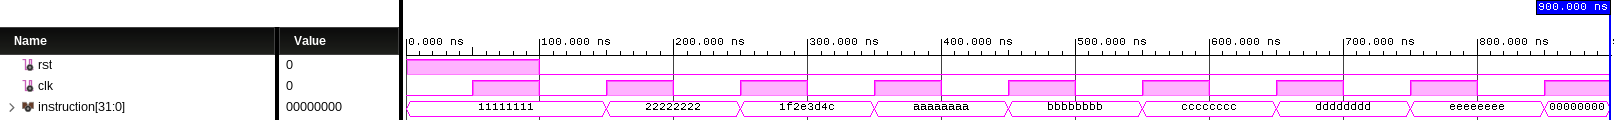
\includegraphics[width=\textwidth]{img/behavior_fetch}
        \caption{Decode stage behavioural simulation}
        \label{fig:behave_fetch}
    \end{figure}

    \begin{figure}[h!]
        \centering
        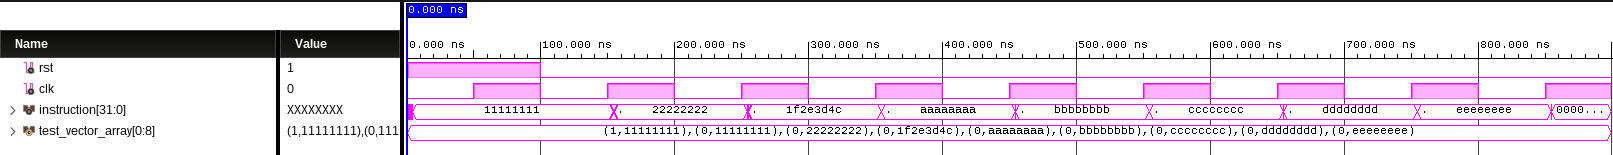
\includegraphics[width=\textwidth]{img/synthesis_fetch}
        \caption{Decode stage post-synthensis timing simulation}
        \label{fig:synth_fetch}
    \end{figure}

    \begin{figure}[h!]
        \centering
        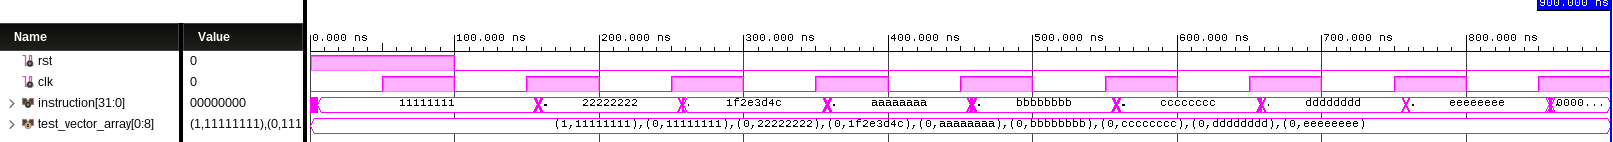
\includegraphics[width=\textwidth]{img/impl_fetch}
        \caption{Decode stage post-implementation timing simulation}
        \label{fig:impl_fetch}
    \end{figure}

    Figures \ref{fig:behave_fetch}, \ref{fig:synth_fetch}, and
    \ref{fig:impl_fetch} correctly show the expected outputs noted
    in Table \ref{tab:inst_mem}. These results are automicatally confirmed
    by the assertions placed in the test bench loop to verify results.
    \\
    It is important to note that the timing delays associated with the Baysis-3
    board were small enough to fit inside a single 100ns clock cycle.
    \\
    The first instruction will stay active for two clock periods because the
    active high reset will keep the program counter at zero. This means
    that it is reading the first instructions twice which is expected.
    
    \pagebreak
    \subsection*{Decode stage}

    The decode stage test bench involves choosing a set of instructions
    and verifying the output of the corresponding control signals.
    
    Because the decode stage also takes in inputs for writing data
    to the registers. This data is output from a previous instruction
    and is passed to the decode stage via following stages.
    
    The following instructions were passed to the decode testbench. The
    set of expected control signals is also noted.
    
    \begin{table}[H]
        \renewcommand{\arraystretch}{1.2}
        % \setlength{\tabcolsep}{12pt}
        \caption{Instruction fetch test cases}
        \begin{center}
            \begin{tabular}{|c|c|c|c|c|c|c|}
                \hline
                Instruction & \code{RegWrite} & \code{MemToReg} & \code{MemWrite} & \code{ALUControl} & \code{ALUSrc} & \code{RegDst}\\\hline
                \hline
               	\code{NOOP} & \code{1} & \code{0} & \code{0} & \code{1100} & \code{0} & \code{1}\\\hline
               	
               	\code{add} & \code{1} & \code{0} & \code{0} & \code{0100} & \code{0} & \code{1}\\\hline
               	
               	\code{addi} & \code{1} & \code{0} & \code{0} & \code{0100} & \code{1} & \code{0}\\\hline
               	
               	\code{ori} & \code{1} & \code{0} & \code{0} & \code{1000} & \code{1} & \code{0}\\\hline
               	
               	\code{sw} & \code{0} & \code{0} & \code{1} & \code{0100} & \code{1} & \code{0}\\\hline
               	
            \end{tabular}
        \end{center}
        \label{tab:decode}
    \end{table}

	The instruction without the operands are shown in Table \ref{tab:decode}.
	This is because the operands are not related to the expected control
	signal values shown in the table.
	
	Using this input data, behavioural, post-synthesis timing, and
	post-implementation timing simulation waveforms were generated.
	
	Assertions were placed inside the testing loop to verify that the
	output signals from the circuit were correct.
	
	\begin{figure}[h!]
        \centering
        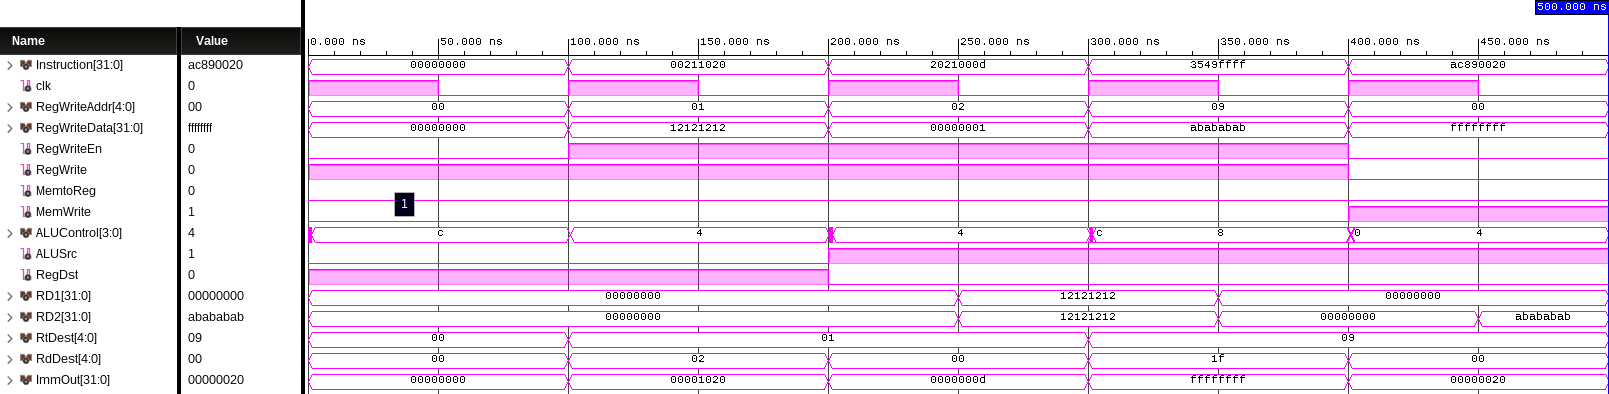
\includegraphics[width=\textwidth]{img/synthesis_decode}
        \caption{Behvioural simulation for decode stage}
        \label{fig:behave_decode}
    \end{figure}

    \begin{figure}[h!]
        \centering
        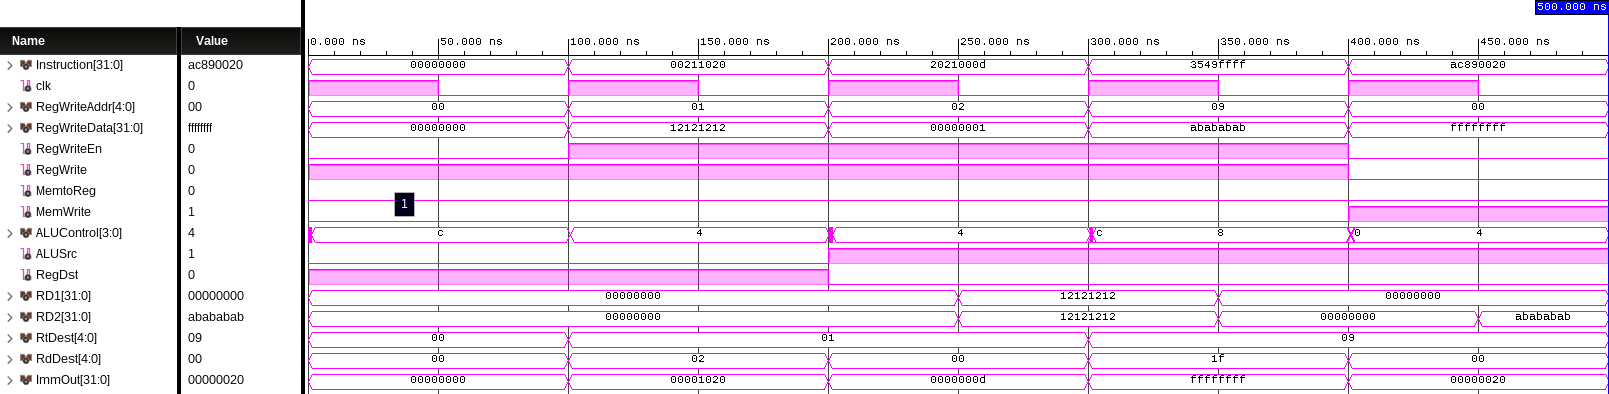
\includegraphics[width=\textwidth]{img/synthesis_decode}
        \caption{Post-synthesis timing simulation for decode stage}
        \label{fig:synth_decode}
    \end{figure}

    \begin{figure}[h!]
        \centering
        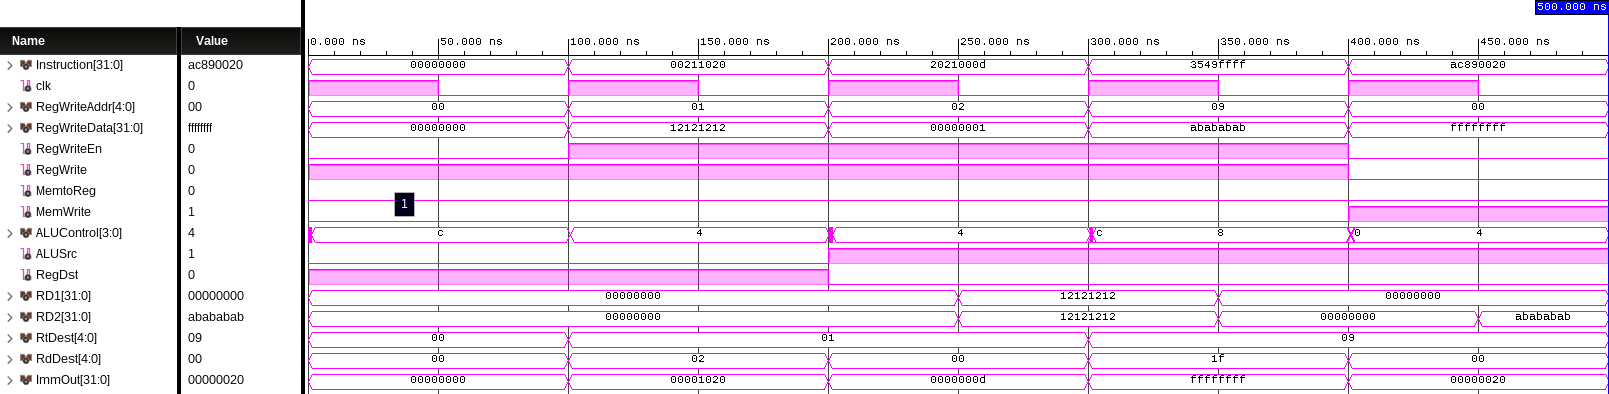
\includegraphics[width=\textwidth]{img/synthesis_decode}
        \caption{Post-implementation timing simulation for decode stage}
        \label{fig:impl_decode}
    \end{figure}

    
    \pagebreak
    
    Looking at the simulation results, the output signals are as expected and
    shown in Table \ref{tab:decode}. There is more being tested in this
    test-bench than depicted in the table. Read data from the register
    file is also asserted. All registers in the register file are initialized
    to zero by default. When certain instructions are executed with
    write data inputs, register data is overwritten.
    
    The final two instructions (\code{ori} and \code{sw}) will sequentially
    write to the \code {\$t1} register followed by a read to verify its outputs.
    Because none of the assertions were tripped, the simulation resulted in
    success indicating a working implementation of the decode stage.
    
    The sign extend functionality was also tested on the \code{ori} instruction.
    The full instruction was \code{ori \$a0 \$a1 0xffff}. The \code{0xffff}
    or \code{-1} would need to be sign-extended into \code{0xffffffff}
    when shown in 32-bit \code{ImmOut} signal. Looking at the second to 
    last testcase, the \code{ImmOut} signal has the correct value. 

    \section*{Conclusion}
    This laboratory exercise introduced the concept of the instruction
    memory and implemented the instruction fetch and decode stages.
    and implemented a generically sized register file.
    The instruction fetch wired an internal program counter to keep track
    of the address of the current instruction and incremented the PC after
    every clock.
    The purpose of the decode stage was to break down the input instruction
    into control signals used by the execute stage later in the architecture.
	This exercise was successful as the design was fully tested and all issues
	found in testbenches were eliminated.

    \pagebreak

    \section*{Demo results}
    
    \subsection*{Fetch}
    \begin{figure}[h!]
        \centering
        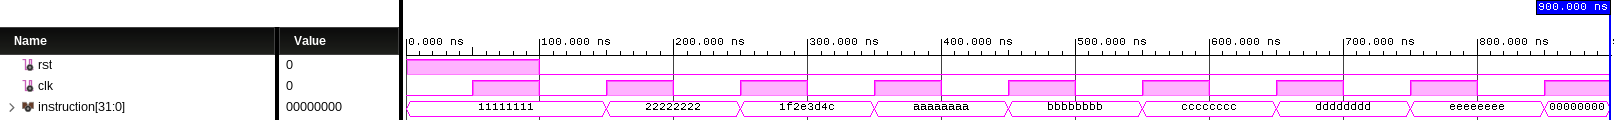
\includegraphics[width=\textwidth]{img/behavior_fetch}
        \caption{Behavioural simulation of Fetch}
        %! suppress = FigureNotReferenced
        \label{fig:demo1}
	\end{figure}
    \begin{figure}[h!]
        \centering
        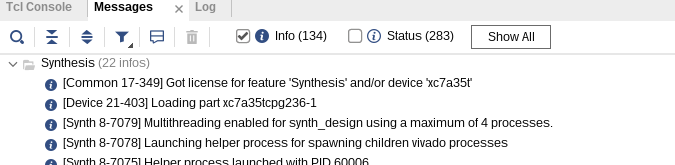
\includegraphics[width=\textwidth]{img/warning_synth_fetch}
        \caption{No warnings generated during synthesis}
        %! suppress = FigureNotReferenced
        \label{fig:demo1}
	\end{figure}
    \begin{figure}[h!]
        \centering
        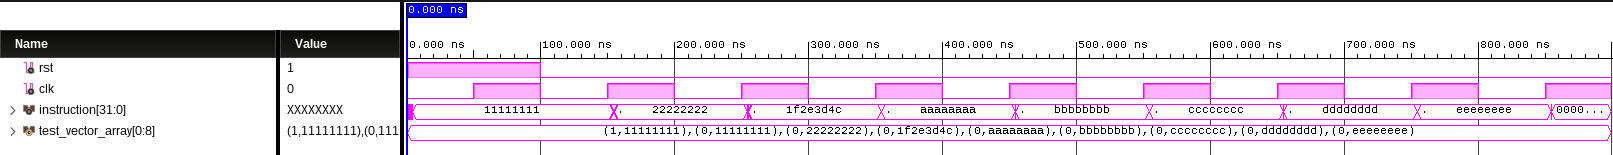
\includegraphics[width=\textwidth]{img/synthesis_fetch}
        \caption{Post-synthesis timing simulation of fetch}
        %! suppress = FigureNotReferenced
        \label{fig:demo1}
	\end{figure}
    \begin{figure}[h!]
        \centering
        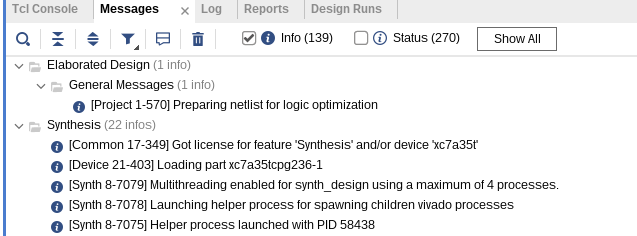
\includegraphics[width=\textwidth]{img/warning_impl_fetch}
        \caption{No warnings generated during implementation}
        %! suppress = FigureNotReferenced
        \label{fig:demo1}
	\end{figure}
    \begin{figure}[h!]
        \centering
        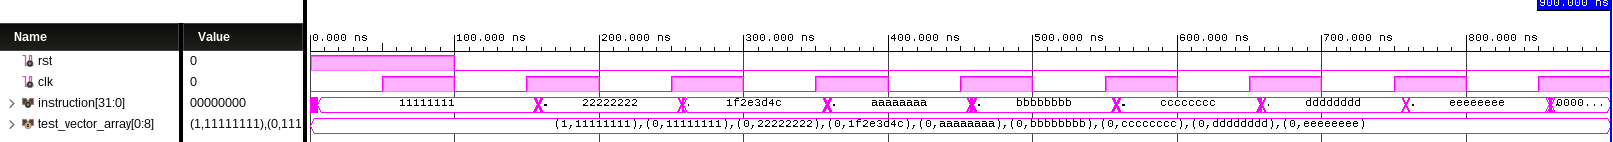
\includegraphics[width=\textwidth]{img/impl_fetch}
        \caption{Post-implementation timing simulation of fetch}
        %! suppress = FigureNotReferenced
        \label{fig:demo1}
	\end{figure}
	
	\pagebreak
	
    \subsection*{Decode}
    \begin{figure}[h!]
        \centering
        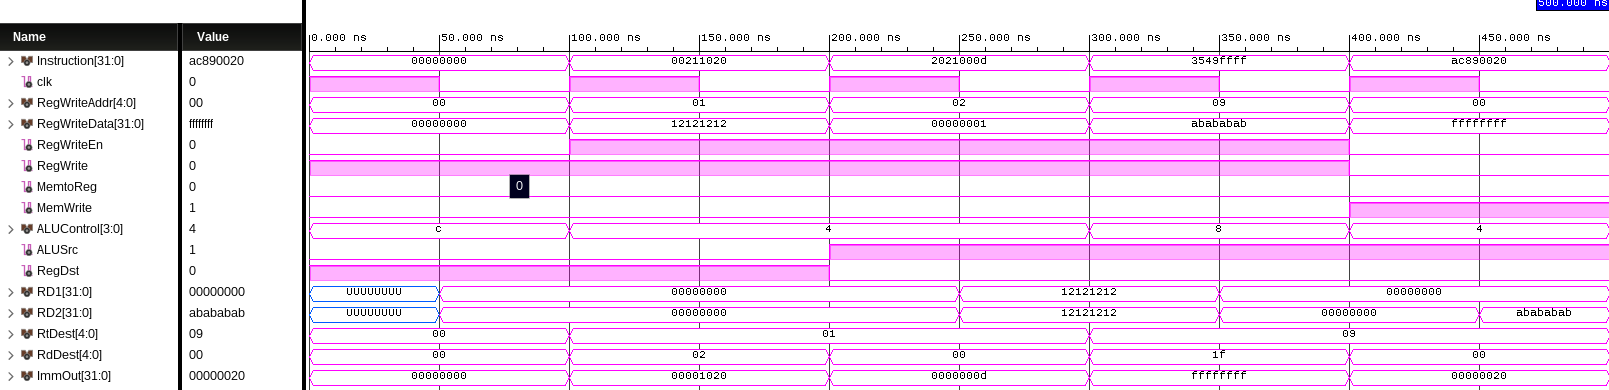
\includegraphics[width=\textwidth]{img/behavior_decode}
        \caption{Behavioural simulation of decode}
        %! suppress = FigureNotReferenced
        \label{fig:demo1}
	\end{figure}
    \begin{figure}[h!]
        \centering
        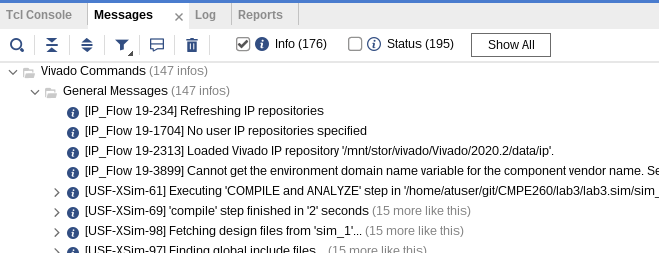
\includegraphics[width=\textwidth]{img/warning_synth_decode}
        \caption{No warnings generated during synthesis}
        %! suppress = FigureNotReferenced
        \label{fig:demo1}
	\end{figure}
    \begin{figure}[h!]
        \centering
        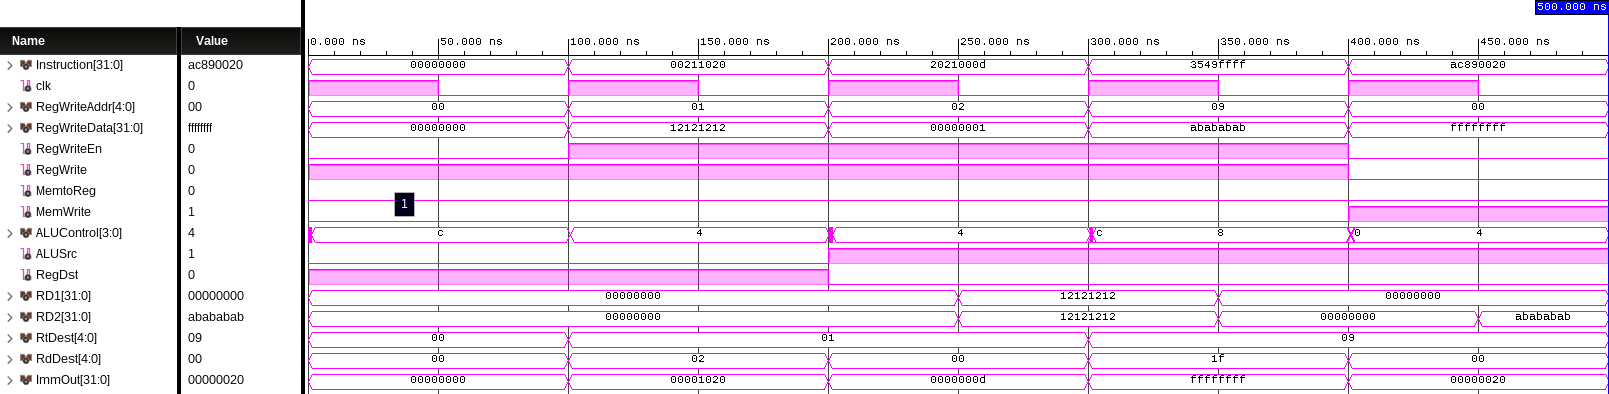
\includegraphics[width=\textwidth]{img/synthesis_decode}
        \caption{Post-synthesis timing simulation of decode}
        %! suppress = FigureNotReferenced
        \label{fig:demo1}
	\end{figure}
    \begin{figure}[h!]
        \centering
        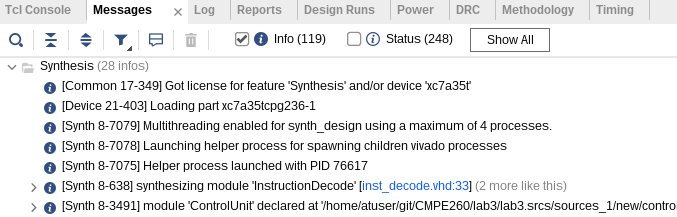
\includegraphics[width=\textwidth]{img/warning_impl_decode}
        \caption{No warnings generated during implementation}
        %! suppress = FigureNotReferenced
        \label{fig:demo1}
	\end{figure}
    \begin{figure}[h!]
        \centering
        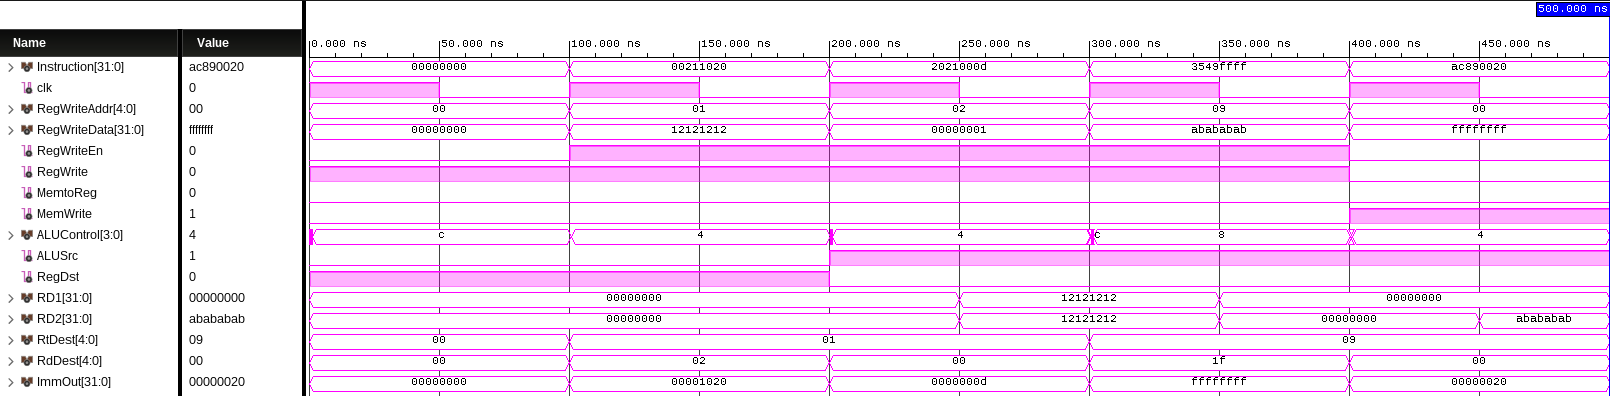
\includegraphics[width=\textwidth]{img/impl_decode}
        \caption{Post-implementation timing simulation of decode}
        %! suppress = FigureNotReferenced
        \label{fig:demo1}
	\end{figure}


\end{document}